%%% Laboratory	 Notes
%%% Template by Mikhail Klassen, April 2013
%%% Contributions from Sarah Mount, May 2014
\documentclass[a4paper]{tufte-handout}

\newcommand{\workingDate}{\textsc{Summer $|$ 2016}}
\newcommand{\userName}{Cail Daley}
\newcommand{\institution}{Leiden University}

\usepackage{lab_notes}


\usepackage{hyperref}
\usepackage{hypcap}
\hypersetup{
    pdffitwindow=false,            % window fit to page
    pdfstartview={Fit},            % fits width of page to window
    pdftitle={HD_100546_Modeling_Notes},     % document title
    pdfauthor={Cail Daley},         % author name
    pdfsubject={},                 % document topic(s)
    pdfnewwindow=true,             % links in new window
    colorlinks=true,               % coloured links, not boxed
    linkcolor=DarkScarletRed,      % colour of internal links
    citecolor=DarkChameleon,       % colour of links to bibliography
    filecolor=DarkPlum,            % colour of file links
    urlcolor=DarkSkyBlue           % colour of external links
}

\title{HD 100546 Modeling}
\date{2016}

\begin{document}
\maketitle

%%%%%%%%%%%%%%%%%%%%%%%%%%%%%%%%%%%%%%%%%%%%%%%%%%%%%%%%
\listoftables
\listoffigures

\hrulefill
%%%%%%%%%%%%%%%%%%%%%%%%%%%%%%%%%%%%%%%%%%%%%%%%%%%%%%%%

\begin{tasks}
    \begin{itemize}
      \item Nada
    \end{itemize}
\end{tasks}

%%%%%%%%%%%%%%%%%%%%%%%%%%%%%%%%%%%%%%%%%%%%%%%%%%%%%%%%

\begin{maybe}
    \begin{itemize}
      \item Spectral profile of outer disk? Use polygon to make a ring, compare to Pineda
      \item PV/spectral profile where blob is?
    \end{itemize}
\end{maybe}

%%%%%%%%%%%%%%%%%%%%%%%%%%%%%%%%%%%%%%%%%%%%%%%%%%%%%%%%

\begin{cath}
    \begin{itemize}
      \item Please note, all tables and figures pertain to the original start velocity uniform CLEAN, NOT the more recent and better-fitting shifted start velocity robust=0.5 CLEAN.
    \end{itemize}

\end{cath}
%%%%%%%%%%%%%%%%%%%%%%%%%%%%%%%%%%%%%%%%%%%%%%%%%%%%%%%%

\newday{2 August 2016}

\mypar{Blob Modelling}
To fit the residual blob, a velocity $v_{blob}$ is set within a radial range $[r_{start}, r_{end}]$ and an azimuthal range $[\phi_{start}, \phi_{end}]$. As the residual blob is roughly the size of the beam, I will use the location of the residual blob to center the model blob, and the beam size to place upper limits on the radial and azimuthal width. The inner companion planet is thought to be \textasciitilde10 AU from the star and one pixel is \textasciitilde11 AU, so there is little motivation for setting the inner radius to anything greater than 0. The best fit position angle for the warp model was 64\textdegree, about 80\textdegree  less than the outer disk position angle of 144\textdegree. The azimuthal angle is measured counterclockwise with respect to the semi-major axis of the disk, with 0 \textdegree  in the upper right corner of the image; thus 80\textdegree  less than the position angle of the outer disk corresponds to an azimuthal angle of 280\textdegree. The beam is .94 x .42; a rough calculation of the inverse tangent of the  width-to-length at maximum width (.47 x .21) gives a total angle of $24*2 \approx 50$\textdegree. \\
As such, I will center the model blob at 280\textdegree, and let the azimuthal angle vary up to 30\textdegree on either side, while also varying the outer radius up to slightly more than the length of one beam, \textasciitilde 100 AU.\\

\hrulefill
%%%%%%%%%%%%%%%%%%%%%%%%%%%%%%%%%%%%%%%%%%%%%%%%%%%%%%%%

\newday{26 July 2016}
Added final results of warp model run; a summary of the model parameters can be found in Table \ref{tab:warp parameters}, and a summary of the best-fitting models in Table \ref{tab:warp best fits}. Figures \ref{fig:warp fit plots} \& \ref{fig:warp models} display fit and model plots.


\hrulefill
%%%%%%%%%%%%%%%%%%%%%%%%%%%%%%%%%%%%%%%%%%%%%%%%%%%%%%%%

\newday{25 July 2016}

Minimum disk radius-- unimportant. Change of \textasciitilde1.2 km/s in quadratic sum for a disk starting at 12 AU (1 pixel), and change of \textasciitilde11.8 km/s for a disk starting at 24 AU (2 pixels). Seems like adding an inner radius won't have much effect if it is to be physically realistic.

\noindent Centered binned residual plot so that middle bin ranges from -0.5 km/s to 0.5 km/s.

\noindent Added isovelocity contours to channel maps and mirror channel plot; aspect ratio of 0.03 is not visibly different from flat disk.

\mypar{A Circumplanetary Disk?}
After meeting with Catherine and Paola, we agree that a warp seems unlikely. Not only do the positive residuals show up exclusively on the negative-velocity side of the disk, they are elongated along the semi-\textit{minor} axis of the disk. A higher inclination is needed to fit the high-velocity blob, but this necessarily  elongates the warp along its semi-\textit{major} axis. Thus the warp can be rotated to eliminate different parts of the residual blob, but it is impossible to remove the entire blob.\\
A possible explanation for this asymmetrical blob is a circumplanetary disk, possibly rotating around the planet candidate at \textasciitilde10 AU. \citep{Walsh14} If part of the disk were hidden behind the planet or obscured by the circumstellar disk, it is conceivable that such a circumplanetary disk could contribute super-keplerian blueshifted emission while the corresponding redshifted emission is obscured. Moving forward, I will increase the velocity values of the unwarped model keplerian velocity field, simulating a half-visible circumplanetary disk, at the location of the blob in an attempt to reproduce the data.



\hrulefill
%%%%%%%%%%%%%%%%%%%%%%%%%%%%%%%%%%%%%%%%%%%%%%%%%%%%%%%%

\newday{20 July 2016}

Reorganized and updated the plots created by the model:
\begin{itemize}
  \item Removed ratio plot; replaced with a version of the residual image binned to the velocity resolution (0.22 km/s)
  \item Added a histogram plotting the number of pixels in each velocity channel bin
  \item Added a quantification of the residual square sum for the outer disk (r>150)

\end{itemize}

\hrulefill
%%%%%%%%%%%%%%%%%%%%%%%%%%%%%%%%%%%%%%%%%%%%%%%%%%%%%%%%

\newday{19 July 2016}

Although a model with a sharp transition is unlikely to be physically realistic, this sharp transition is effectively smoothed during the convolution process and thus does not significantly differ from a more smooth inclination prescription. Additionally, the inclination power law of Equation \ref{eq:rosenfeld i} becomes significantly harder to implement when both position angle and inclination vary with radius.  Models with a sharp transition will thus be used in this stage of the warp modeling as they are much simpler.

\hrulefill
%%%%%%%%%%%%%%%%%%%%%%%%%%%%%%%%%%%%%%%%%%%%%%%%%%%%%%%%

\newday{6 July 2016}

In amom.py, aspect ratio is defined as $\frac{4H_p}{r}$, where $H_p$ is the pressure scale height.

\newthought{Adding Warp:}\\
I wrote a script, analytical\_warp.py, to create an analytical models of a warped disk using HD 100546's spatial grid. This script will plot offset as a function of radius in one-dimensional profile slices as well as two-dimensional heat maps. Models without a warp have failed to fit the data primarily within \textasciitilde0.27", or 26 AU of the star, suggesting that the warp is most significant within this area. A model with a sharp transition between inclinations at the location of the warp (i.e. discontinuous) is unlikely to fit the disk well, and as the spatial resolution of the ALMA observations is \textasciitilde12 AU, it is ungainly and nearly impossible to create a model with two separate inclinations and a smooth ``transition band'' in between. As such, I will be skipping straight to Katherine Rosenfeld's \citep{Rosenfeld12} 2012 prescription for a power-law inclination profile:

\begin{equation}
  \label{eq:rosenfeld i}
  i(r)=i_0(\frac{r}{r_0})^{-y}
\end{equation}

\mypar{Inclination Power Law: Positive or Negative Second Derivative?}
\label{par:power law}
In this equation, inclination decreases with radius. The unwarped models with the smallest peak residuals seem to prefer lower inclinations and position angles, as these values better fit the positive residual blob close to the center of the disk that can be seen in the residual image of Figure \ref{fig:no warp models}). As this blob is close to the center of the disk, this suggests that the inner disk has a lower inclination than the outer. \\
However, I suspect that this is the wrong conclusion. As the resdual blob is positive, the model is \textit{underpredicting} the data, i.e. the model velocities at the location of the blob are lower than those of the data. Given the available parameter space of an unwarped disk, the best fit solution seems to involve rotating the disk so that the high-velocity areas along the semi-major axis lie closer to the blob, and then decreasing the inclination of the disk so as to mitigate the effects of this rotation on other parts of the disk. This effect becomes evident when the peak best fits are compared to the sum best fits: the peak best fits, sensitive only to the largest residual, prefer lower position angles and inclinations (130, 30) than the sum best fits (144, 36) which are more sensitive to overall fit. \\
This is all to say that even though the best-fit models prefer a lower inclination, indicating a disk with an inclination power law profile that increases with radius, the positive residual blob in the inner parts of the disk may more strongly suggest a decreasing power law as described by Rosenfeld.



\hrulefill

%%%%%%%%%%%%%%%%%%%%%%%%%%%%%%%%%%%%%%%%%%%%%%%%%%%%%%%%

\newday{5 July 2016}

\newthought{Started taking notes on modeling work}


\hrulefill
%%%%%%%%%%%%%%%%%%%%%%%%%%%%%%%%%%%%%%%%%%%%%%%%%%%%%%%%


\section{Work Overview (so far)}
\label{sec:Work Overview}

This summer I have been using the script amom.py (jointly written by Catherine Walsh and Atilla Juhasz) to model the first moment map of HD 100546. This is done with the help of a front end, exectute\_amom.py, that reads in the disk's first moment map, creates an ideal model given certain parameters, and then convolves the model with the ALMA image's beam. Unwarped model parameter information for can be found in Table \ref{tab: no warp parameters}.


\subsection{Model Gridding}
execute\_amom.py creates a model for each possible permutation of a set of parameters. For each model, a plot is saved containing five images:
\begin{enumerate}
  \item ALMA data first moment map
  \item Convolved model first moment map
  \item Residuals $(data-model)$
  \item Residuals binned to the velocity resolution, 0.22 km/s.
  \item Histogram of the number of pixels at each velocity, binned to the channel width, 0.11 km/s.
\end{enumerate}

\paragraph{A Note on Residuals}
As the first moment map contains both positive and negative values, the residuals can be somewhat misleading. Positive resdiduals in parts of the disk corresponding to a positive velocity indicate that the model underestimates the data; however, in parts of the disk corresponding to a \textit{negative} velocity, positive resdiduals indicate that the model \textit{oversetimates} the data. To mitigate this potential source of confusion, the signs of residuals in parts of the disk corresponding to a negative veloctiy have been flipped so that positive residuals always suggest that the model is too weak, and negative residuals always suggest that the model is too strong.

For each combination of aspect ratio and cone, a plot (referred to from now on as a ``fit plot'') is saved containing the fit statistics of each model in a matrix of position values and inclinations. Position angle currently ranges between 130 and 160, and inclination ranges between 30 and 60. Two goodness of fit quantifications are used: a $\chi^2$ with $\sigma=1$ (i.e. $\sum(data-model)^2$), and the peak (absolute magnitude) residual. The sum of squares tends to be better for assessing overall goodness of fit, while the peak reveals where and how badly the model fails to fit the data. The models with the smallest sums of squares and smallest peaks are summarized in Tables \ref{tab:no warp best fits} and \ref{tab:no warp best fits}, respectively. Fit plots and best fit models for aspect ratios 0 \& 0.02 are included in Figures \ref{fig:no warp fit plots} and  \ref{fig:no warp models}.


\begin{table}[!p]
\label{tab: no warp parameters}
\centering
\caption[No Warp Model Parameters]{Model parameters (without warp). }
\begin{tabular}{lrr}
  \hfill & Range (\textdegree) &	 Best Fit(\textdegree)\\
  \midrule
  Height Angle &	0, 27&	2\\
  Position Angle &	130, 160 & 144\\
  Inclination     & 30, 60 &	 36\\
\end{tabular}
\end{table}

\leavevmode \newline
\vspace*{2 cm}
\leavevmode \newline

\begin{table}[!p]
  \label{tab:no warp best fits}
  \caption[No Warp Best Fit Model Information]{Best-fitting models without a warp, quantified using sum of squares and peak residual.}
  \begin{tabu} to \textwidth {X[r]X[r]X[r]X[r]X[r]}
    \toprule
    Aspect Ratio & Cone    & Position Angle & Inclination & Sum of Squares\\
    \midrule
    0            &	N/A    & 144         & 36          &	76.59          \\
    0.01         &	Lower  & 144         & 36          &	76.22          \\
    0.01         &	Upper  & 144         & 36          &	77.17          \\
    0.02         &	Lower  & 144         & 36          &	\textbf{76.05} \\
    0.02         &	Upper  & 144         & 36          &	77.95          \\
    0.03         &	Lower  & 144         & 36          &	76.08          \\
    0.03         &	Upper  & 144         & 36          &	78.93          \\
    0.04         &	Lower  & 144         & 36          &	76.31          \\
    0.04         &	Upper  & 144         & 36          &	80.13          \\
    0.1          &	Lower  & 144         & 34          &	81.00          \\
    0.1          &	Upper  & 144         & 34          &	91.64          \\
    0.2          &	Lower  & 144         & 34          &	102.79         \\
    0.2          &	Upper  & 142         & 34          &	124.51         \\
  \end{tabu}

  \vspace*{1 cm}

  \begin{tabu} to \textwidth {X[r]X[r]X[r]X[r]X[r]X[r]}
    \toprule
    Aspect Ratio & Cone & Position Angle & Inclination &	Peak Offset   & Peak Residual\\
    \midrule
    0          & N/A  & 130        & 30        & $(0.24, 0.12)$ &	1.31\\
    0.01       & Lower& 130        & 30        & $(0.24, 0.12)$ &	1.32\\
    0.01       & Upper& 130        & 30        & $(0.24, 0.12)$ &	1.31\\
    0.02       & Lower& 130        & 30        & $(0.24, 0.12)$ &	1.32\\
    0.02       & Upper& 130        & 30        & $(0.24, 0.12)$ &	1.31\\
    0.03       & Lower& 130        & 30        & $(0.24, 0.12)$ &	1.32\\
    0.03       & Upper& 130        & 30        & $(0.24, 0.12)$ &	1.31\\
    0.04       & Lower& 130        & 30        & $(0.24, 0.12)$ &	1.32\\
    0.04       & Upper& 130        & 30        & $(0.24, 0.12)$ &	1.31\\
    0.1        & Lower& 130        & 30        & $(0.24, 0.12)$ &	1.34\\
    0.1        & Upper& 130        & 30        & $(0.24, 0.12)$&\textbf{1.29}\\
    0.2        & Lower& 130        & 30        & $(0.24, 0.12)$ &	1.36\\
    0.2        & Upper& 158        & 30        &$(0.96, -0.36)$ &	-1.30\\
    0.3        & Lower& 158        & 30        &$(-1.32, 0.24)$ &	-1.57\\
    0.3        & Upper& 158        & 30        &$(1.08, -0.24)$ &	-1.45\\
  \end{tabu}
\end{table}


\begin{figure}[!p]
  \label{fig:no warp fit plots}
  \centering
  \caption[No Warp Fit Plots]{Fit plots for models without a warp. \newline
  \noindent \textbf{Left:} Flat disk. \newline
  \noindent \textbf{Right:} Best fit aspect ratio $\frac{4H_p}{r}=0.02$. \newline
  \noindent The difference between a flat disk and the best fit aspect ratio is negligible.}
  \begin{minipage}{.5\textwidth}
    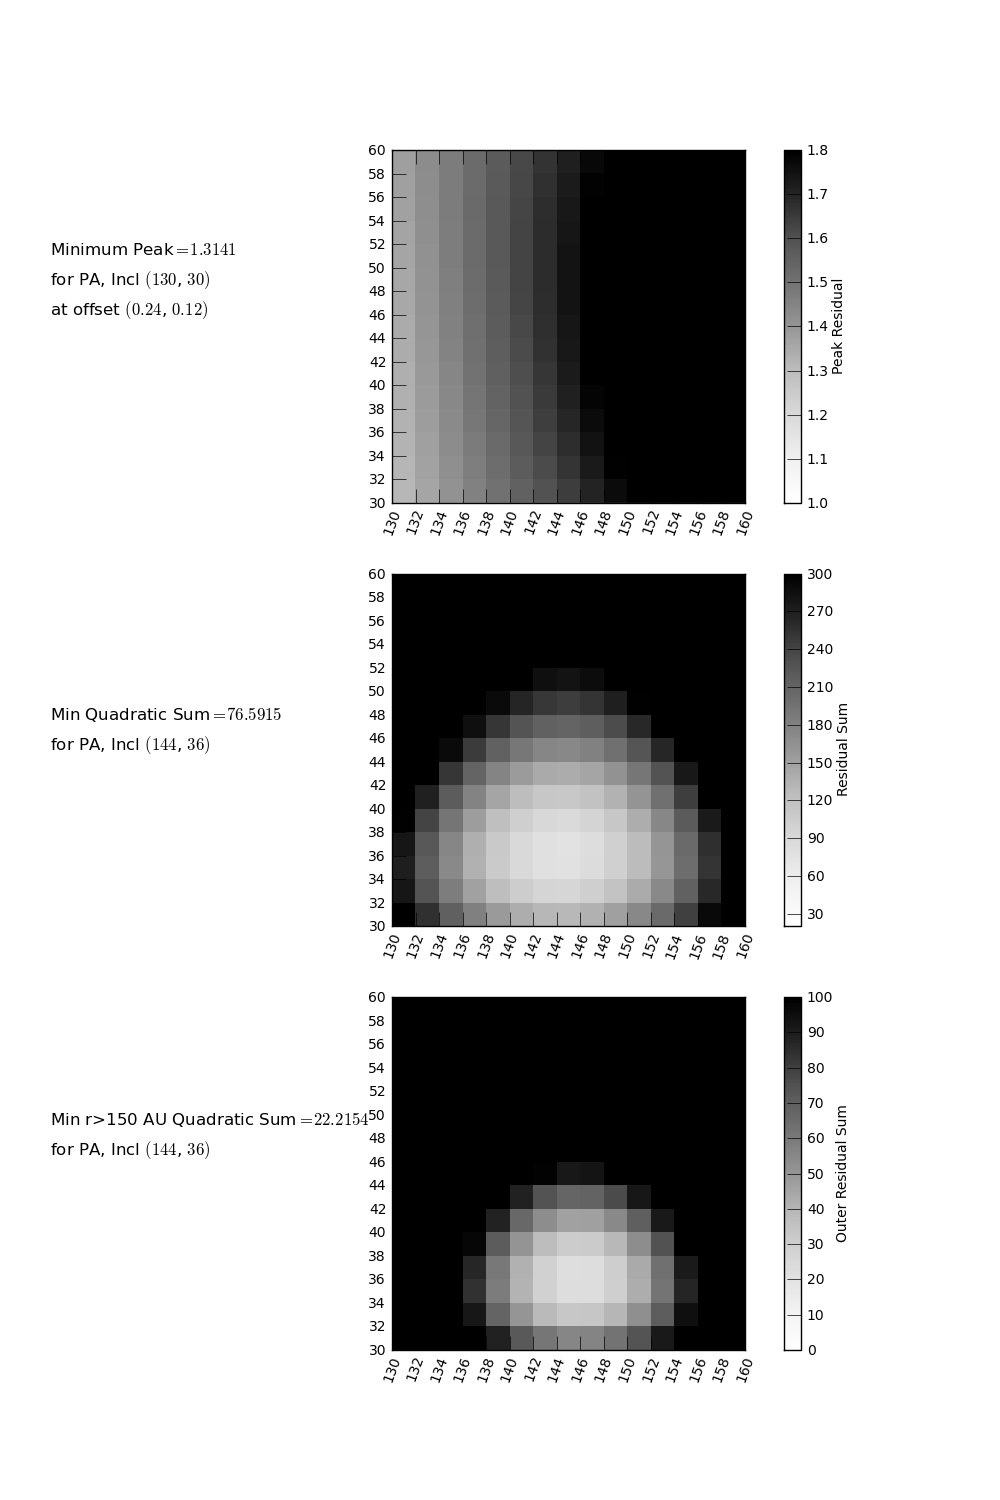
\includegraphics[width=\linewidth]{fit_plot_flat}
  \end{minipage}%
  \begin{minipage}{.5\textwidth}
    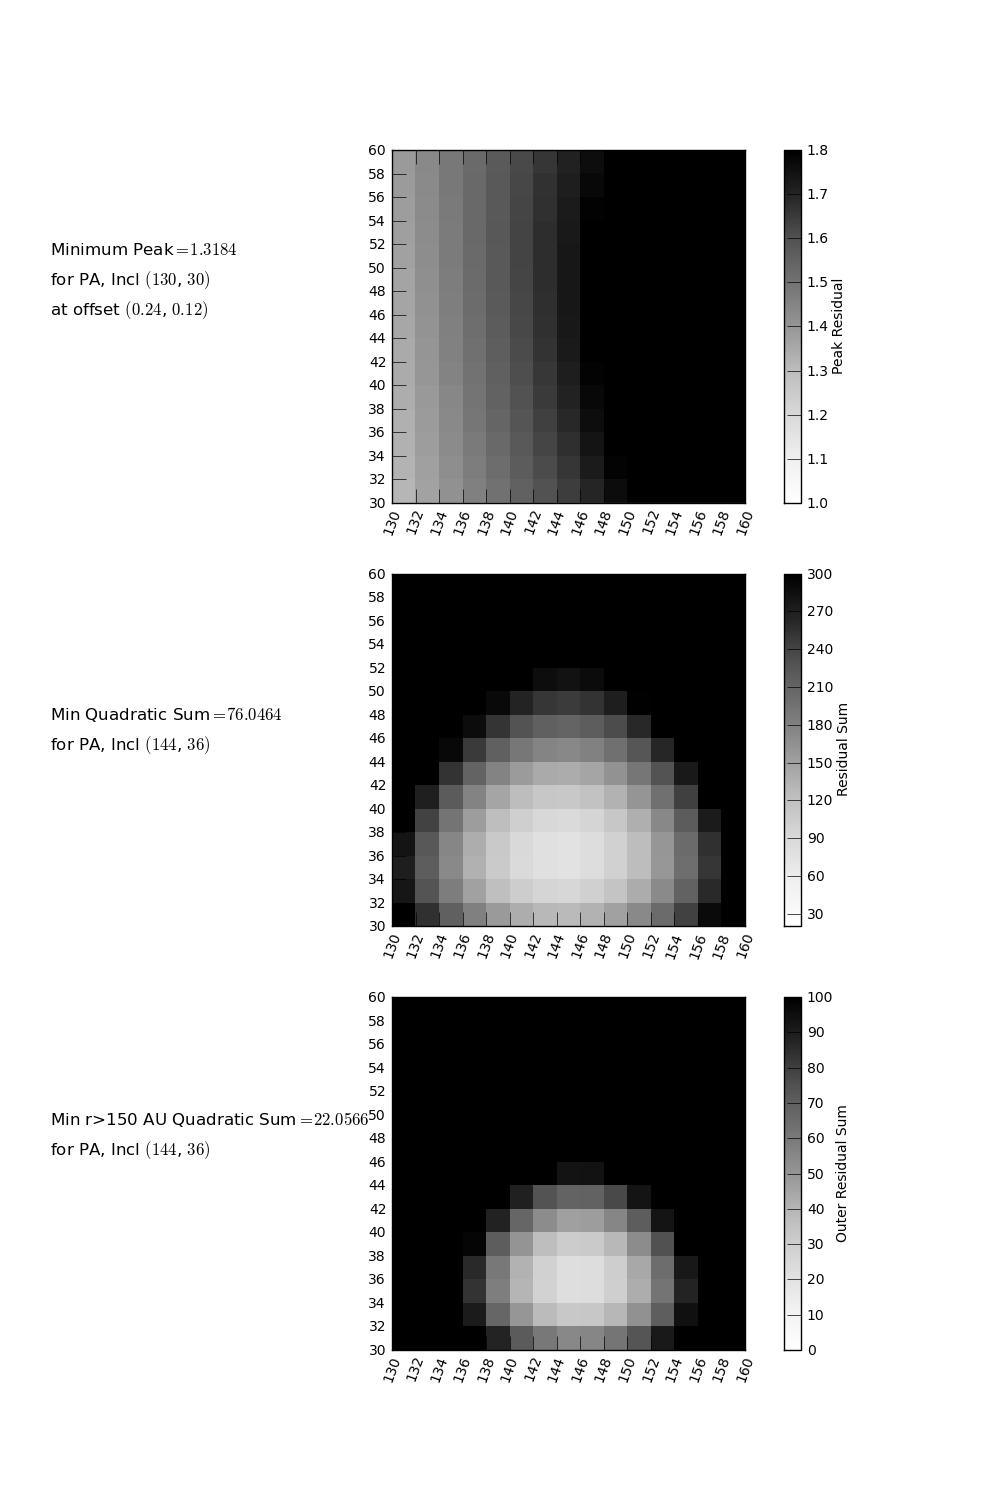
\includegraphics[width=\linewidth]{fit_plot_aspect_0dot02.png}
  \end{minipage}
\end{figure}

\begin{figure}[!p]
  \label{fig:no warp models}
  \centering
  \caption[No Warp Best Fit Models]{Models without a warp. \newline
  \noindent \textbf{Left:} Best fit model for a flat disk. \newline
     Aspect=0 \newline
     Cone=N/A \newline
     Position Angle=144 \newline
     Inclination=36 \newline
   \noindent \textbf{Right:} Best fit model overall. \newline
     Aspect=0.02 \newline
     Cone=Lower \newline
     Position Angle=144 \newline
     Inclination=36 \newline}
  \begin{minipage}{.5\textwidth}
    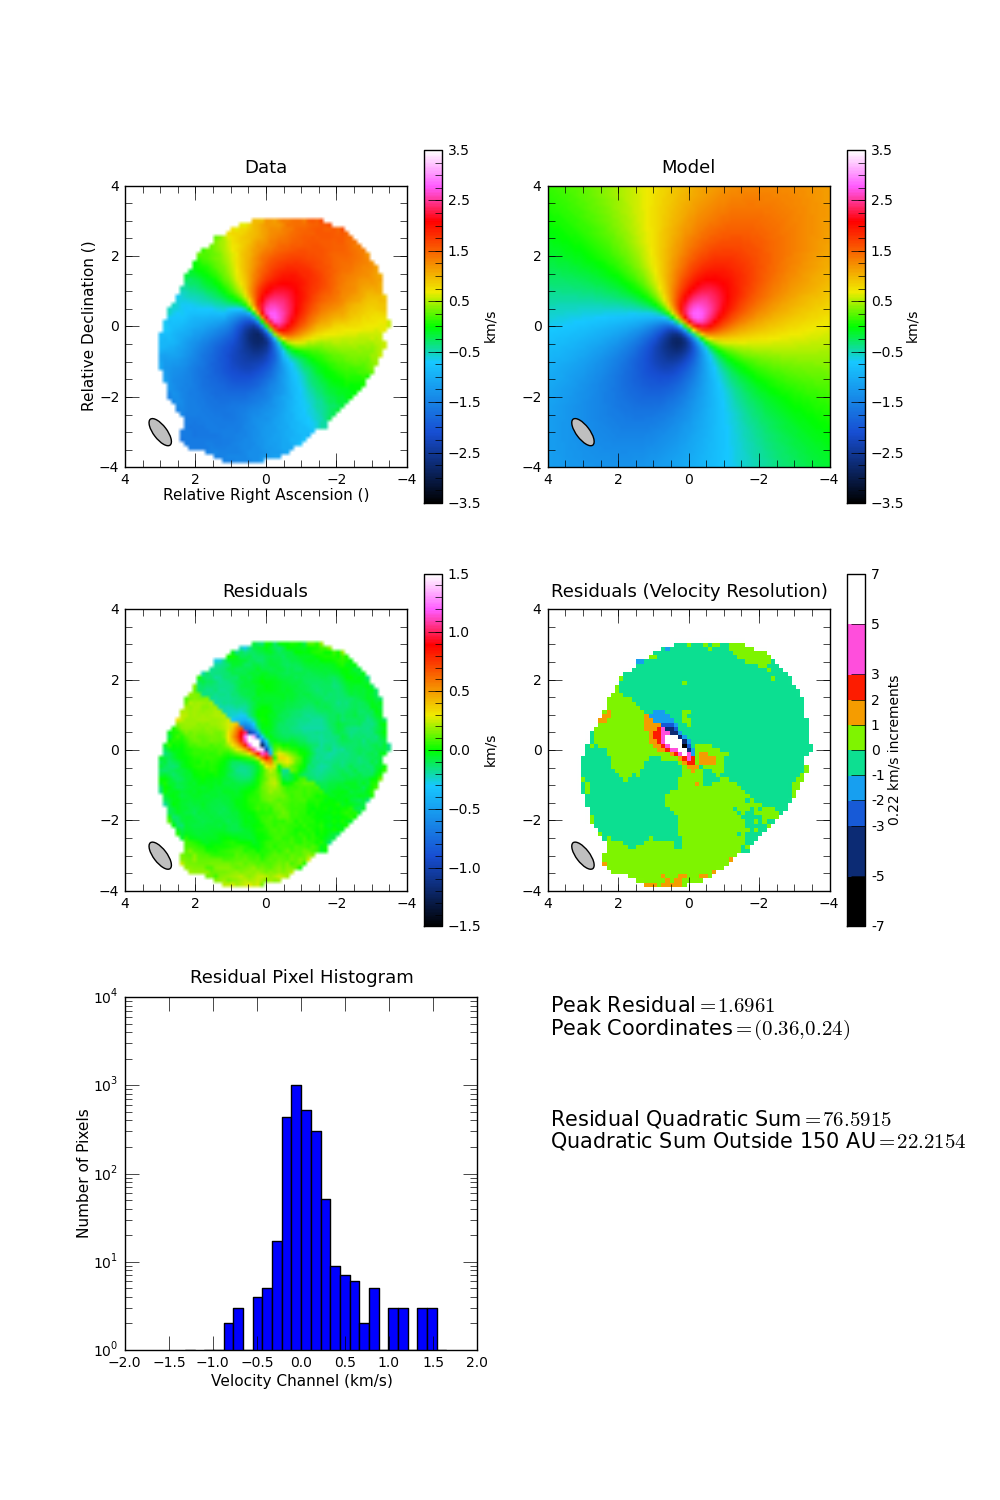
\includegraphics[width=\linewidth]{no_warp_best_fit_flat}
  \end{minipage}%
  \begin{minipage}{.5\textwidth}
    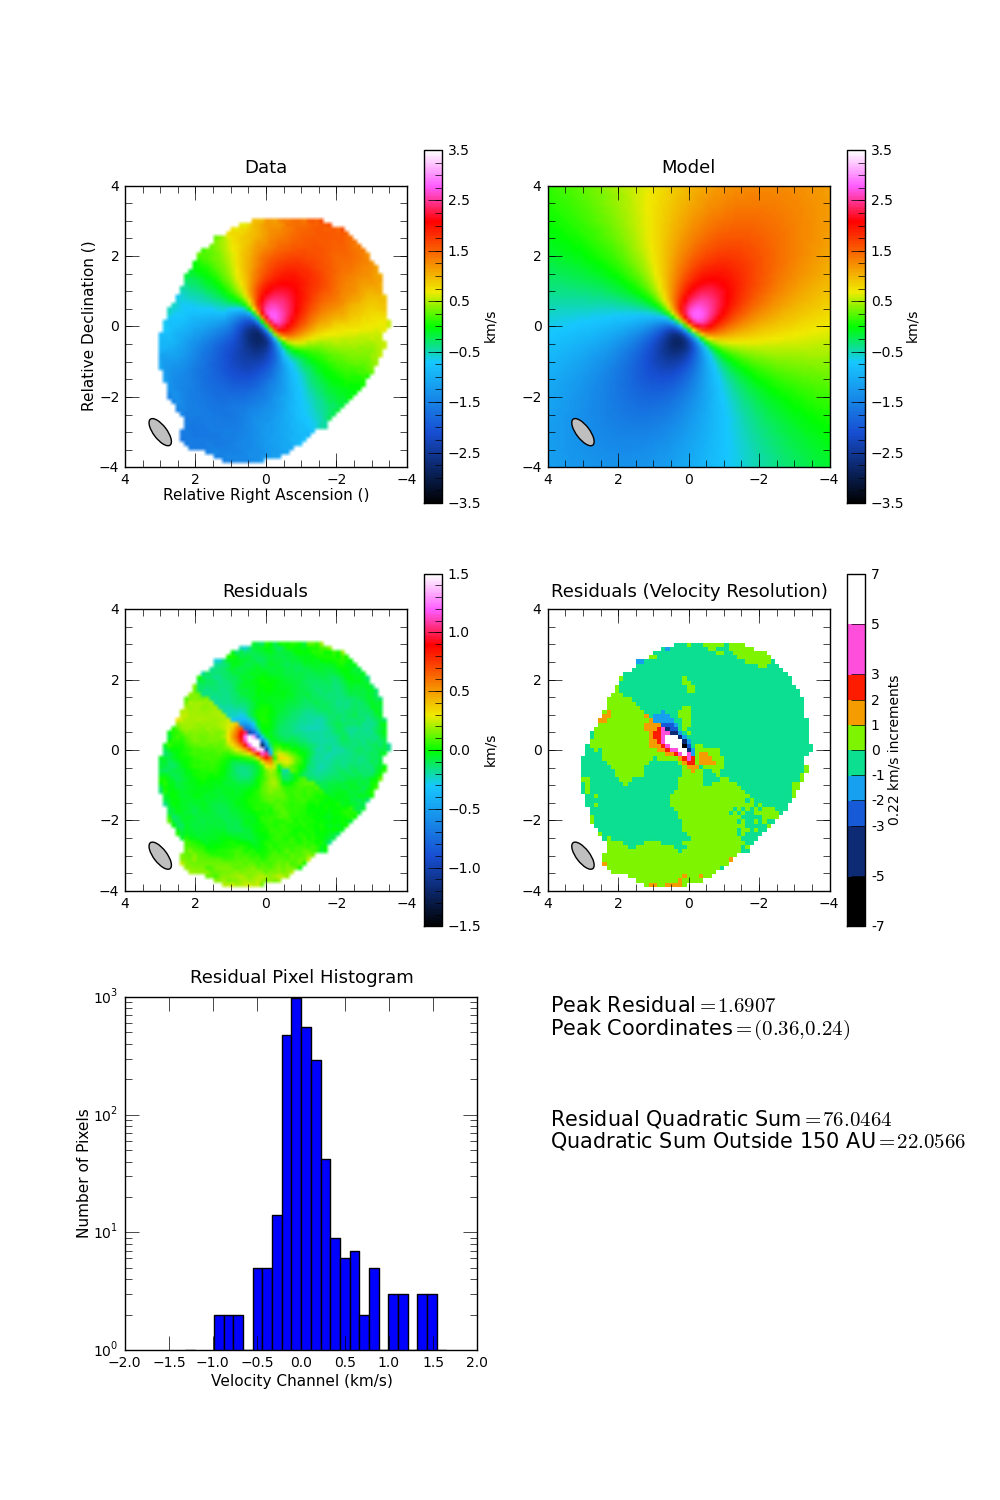
\includegraphics[width=\linewidth]{no_warp_best_fit_aspect_0dot02.png}
  \end{minipage}
\end{figure}

\begin{table}[!p]
\label{tab:warp parameters}
\centering
\caption[Warp Model Parameters]{Model parameters (with warp). }
\begin{tabular}{lrr}
  \toprule
  Parameter 	        &	Start Value              &	 Preferred Value\\
  \midrule
  Stellar Mass              &	2.5 \citep{Manoj06}      &	N/A\\
  Distance (parsecs)        &	96.9 \citep{Meeus12}     &	N/A\\
  Aspect Ratio              &	0.0                      &	N/A\\
  Outer Position Angle      &	144                      &	N/A\\
  Outer Inclination         &	36                       &	N/A\\
  Inner Position Angle      &	55                       &	64\\
  Inner Inclination         &	55                       &	76\\
  Transition Radius (AU)    &	25                    &	60\\
\end{tabular}
\end{table}

\begin{table}[!p]
  \label{tab:warp best fits}
  \caption[Warp Best Fit Model Information]{The best-fitting warp models for each transition radius, quantified using sum of squares and peak positive residual. The positive peak reveals the extent to which the model is capable of eliminating the residual blob. Outer position angle and inclination are fixed at 144 and 36 degrees respectively.}
  \begin{tabu} to \textwidth {X[r]X[r]X[r]X[r]}
    \toprule
    Transition Radius & Inner Position Angle & Inner Inclination & Sum of Squares\\
    \midrule
    10 AU             & 60                   & 36                & 76.59 \\
    20 AU             & 76                   & 52                & 69.78 \\
    30 AU             & 72                   & 60                & 62.71 \\
    40 AU             & 72                   & 56                & 58.32 \\
    50 AU             & 76                   & 64                & 57.23 \\
    60 AU             & 64                   & 76                & \textbf{56.95} \\
    70 AU             & 68                   & 76                & 58.77 \\
    80 AU             & 126                  & 36                & 62.19 \\
    90 AU             & 130                  & 36                & 63.10 \\
  \end{tabu}

  \vspace*{1 cm}

  \begin{tabu} to \textwidth {X[r]X[r]X[r]X[r]X[r]}
    \toprule
    Transition Radius & Inner Position Angle & Inner Inclination & Peak Offset & Peak Positive Residual\\
    \midrule
    10 AU      & 60         & 36       & $(0.36, 0.24)$     &	1.70\\
    20 AU      & 60         & 56       & $(0.24, 0.12)$     &	1.43\\
    30 AU      & 60         & 56       & $(0.24, 0.12)$     &	1.28\\
    40 AU      & 100        & 40       & $(0.24, 0.12)$     &	1.24\\
    50 AU      & 72         & 72       & $(0.24, 0.12)$     &	1.24\\
    60 AU      & 110        & 48       & $(0, -0.12)$       &	1.24\\
    70 AU      & 118        & 40       & $(0.12, 0)$        &	1.24\\
    80 AU      & 116        & 52       & $(0, -0.12)$       &	1.24\\
    90 AU      & 120        & 48       & $(0.12, 0)$        &	1.24\\
  \end{tabu}
\end{table}

\begin{figure}[!p]
  \label{fig:warp fit plots}
  \centering
  \caption[Warp Fit Plots]{Fit plots for warp models. \newline
  \noindent \textbf{Left:} Best fit transition radius $r_0=60$ AU. \newline
  \noindent \textbf{Right:} Transition radius $r_0=90$ AU.}
  \begin{minipage}{.5\textwidth}
    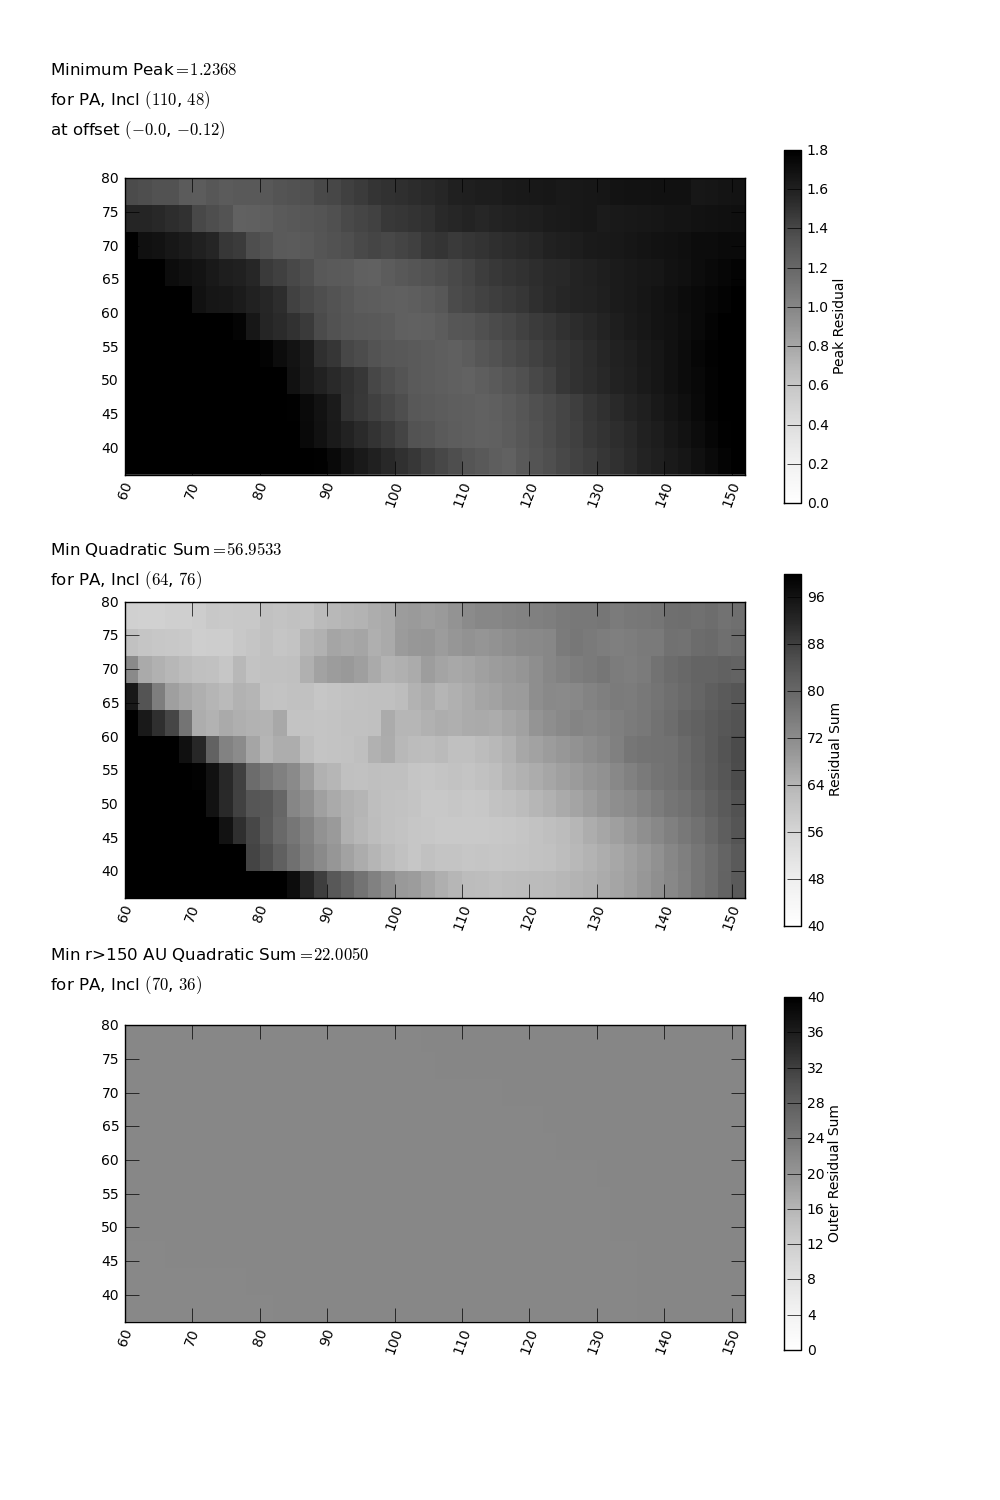
\includegraphics[width=\linewidth]{warp_fit_plot_r0_60}
  \end{minipage}%
  \begin{minipage}{.5\textwidth}
    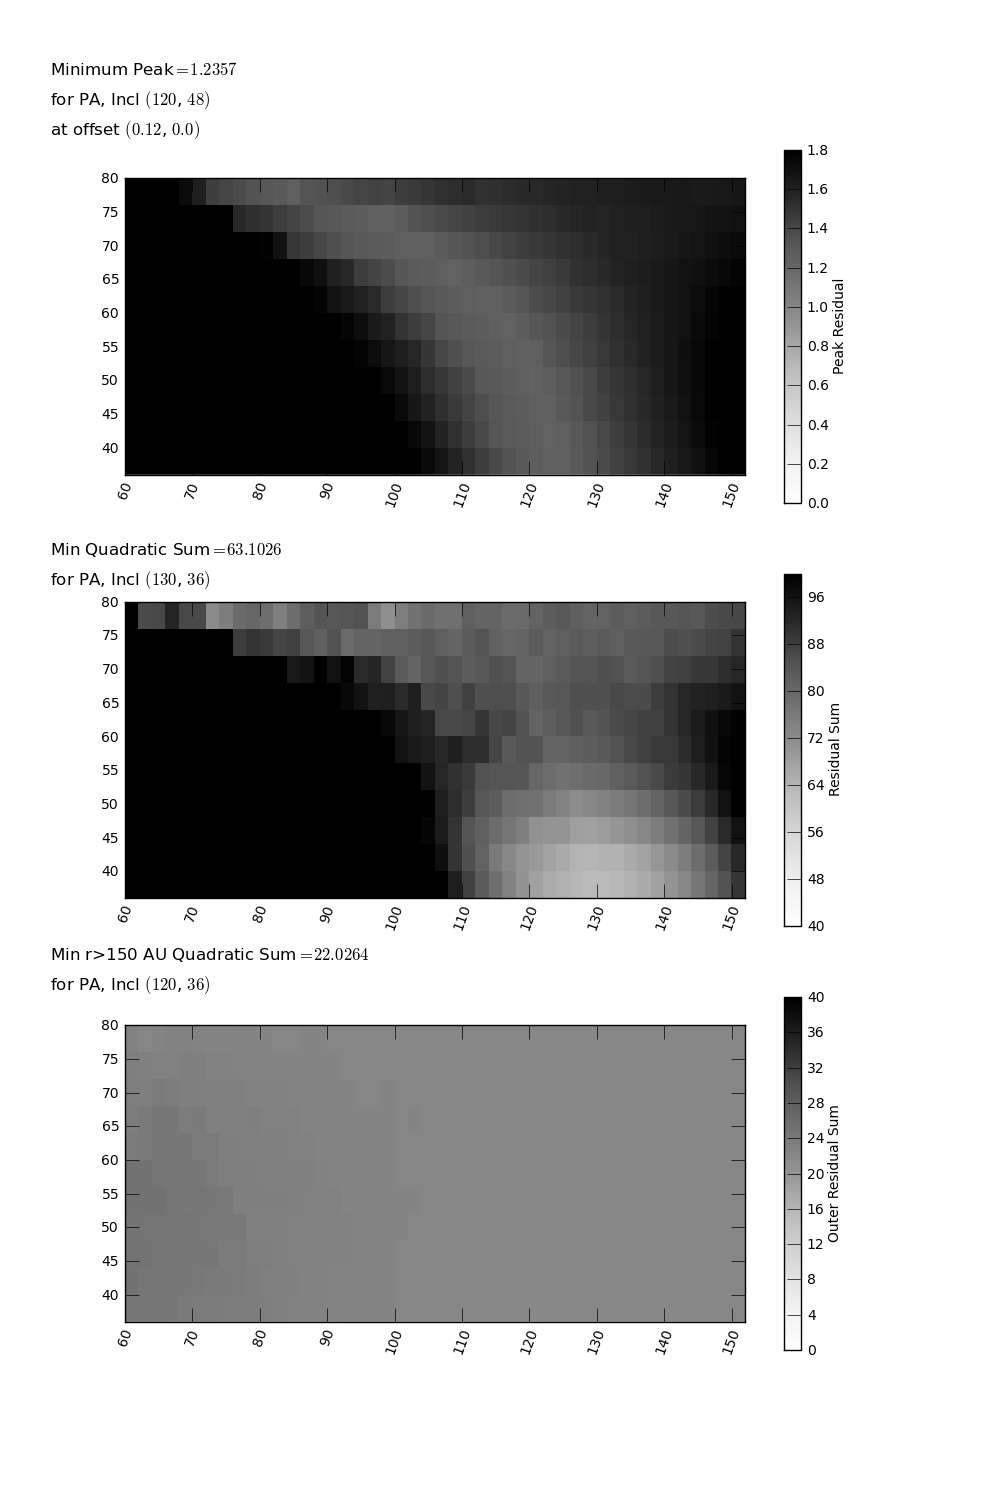
\includegraphics[width=\linewidth]{warp_fit_plot_r0_90}
  \end{minipage}
\end{figure}

\begin{figure}[!p]
  \label{fig:warp models}
  \centering
  \caption[Warp Best Fit Model]{Best fit warp model. \newline
     Aspect=0 \newline
     Cone=N/A \newline
     Transition Radius=60 AU \newline
     Inner Position Angle=64 \newline
     Inner Inclination=76 \newline
     Outer Position Angle=144 \newline
     Outer Inclination=36 \newline
  \noindent \textbf{Left:} Best fit warp model with the model image convolved. \newline
  \noindent \textbf{Right:} Best fit warp model with the model image left unconvolved, revealing the shape of the warp. The binned residual plot has also been redone so that the middle bin is centered around zero, making it easier to assess where the model actually deviates from the data.}
  \begin{minipage}{.5\textwidth}
    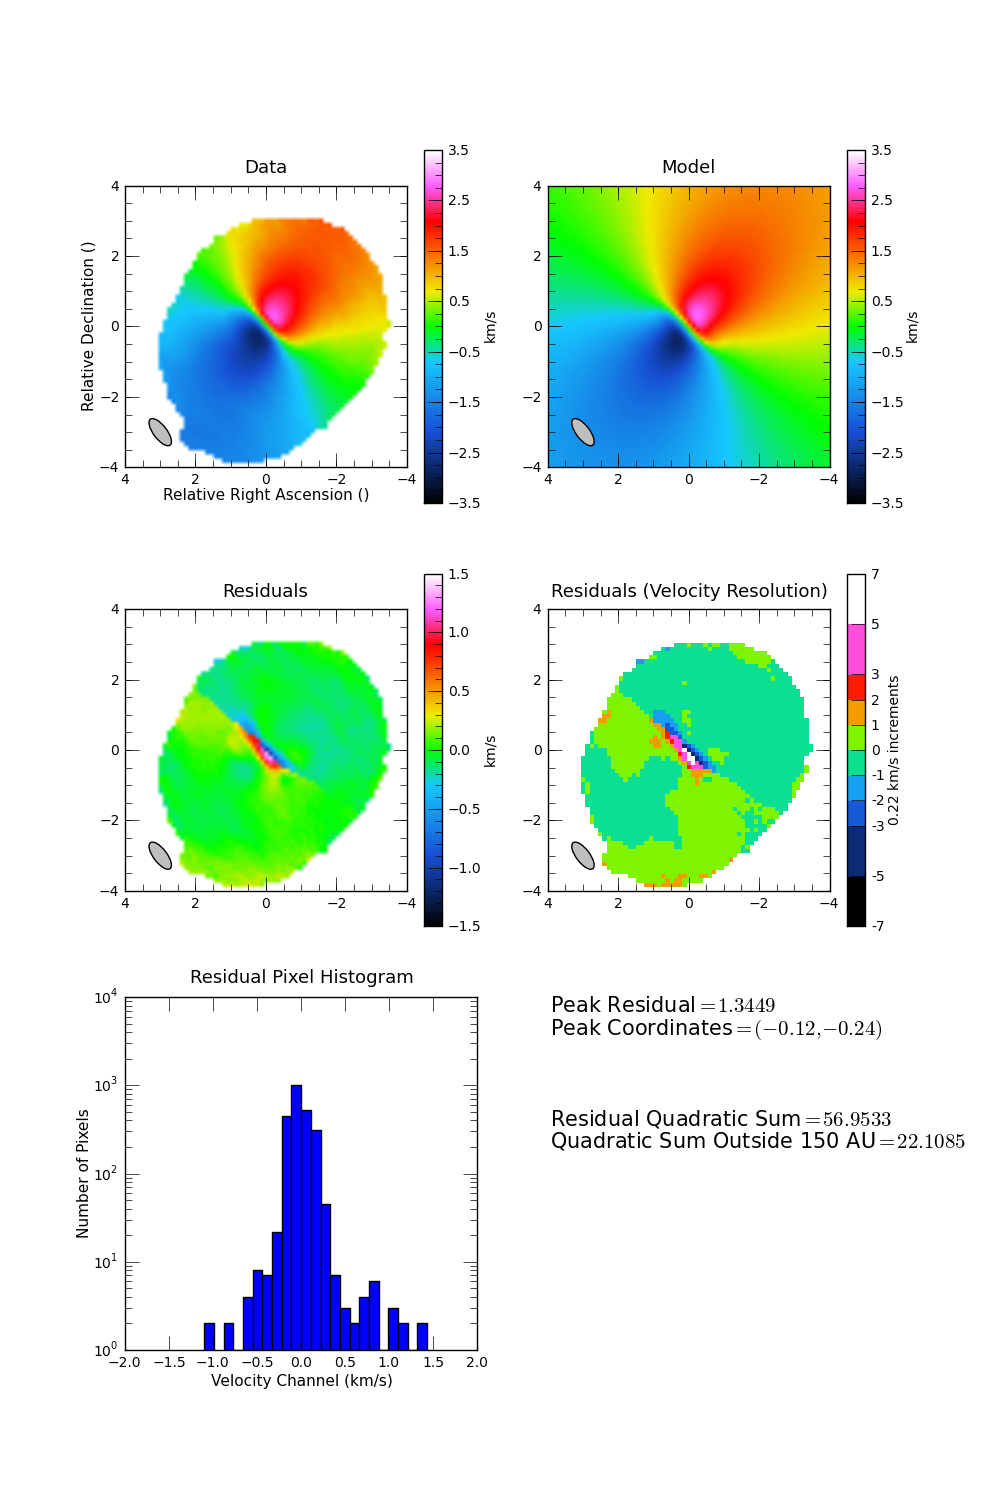
\includegraphics[width=\linewidth]{warp_best_fit_convolved}
  \end{minipage}%
  \begin{minipage}{.5\textwidth}
    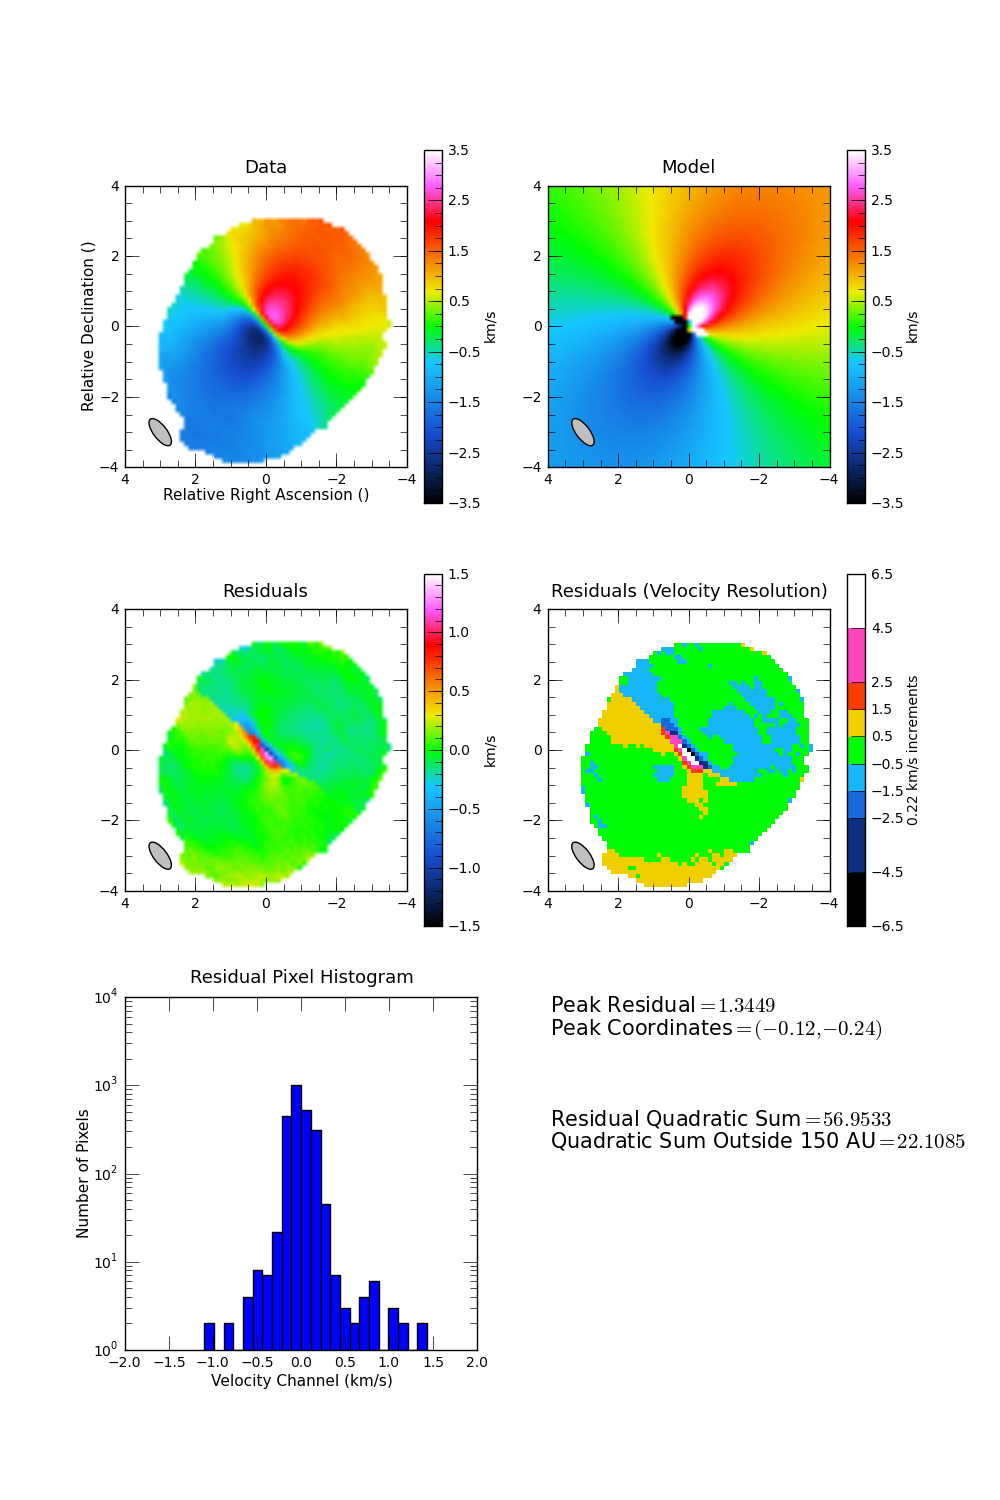
\includegraphics[width=\linewidth]{warp_best_fit_no_convolution}
  \end{minipage}
\end{figure}
\clearpage
%%%%%%%%%%%%%%%%%%%%%%%%%%%%%%%%%%%%%%%%%%%%%%%%%%%%%%%%

\newpage
\bibliographystyle{unsrt}
\bibliography{lab_notes}

\end{document}
